% **************************************************
% Document class
% **************************************************

\documentclass[
	a4paper,
	12pt,
	bibliography=numbered,
	listof=totoc,
	titlepage
]{scrartcl}


% **************************************************
% Settings
% **************************************************

\usepackage{settings}


% **************************************************
% Variables
% **************************************************

\newcommand*{\getUniversity}{Hochschule für angewandte Wissenschaften München}
\newcommand*{\getFaculty}{Fakultät für Informatik und Mathematik}
\newcommand*{\getTitle}{Entwurf und Bereitstellung von Microservices mit Kubernetes am Beispiel eines CRM-Systems}
\newcommand*{\getAuthor}{Simon Hirner}
\newcommand*{\getEmailAddress}{simon.hirner@hm.edu}
\newcommand*{\getMatriculationNumber}{02607918}
\newcommand*{\getCourse}{Wirtschaftsinformatik}
\newcommand*{\getDoctype}{Exposé zur Bachelorarbeit}
\newcommand*{\getSupervisor}{Prof. Dr. Torsten Zimmer}
\newcommand*{\getSubmissionDate}{\today}


% **************************************************
% PDF Metadata
% **************************************************

\hypersetup{
	pdftitle = \getTitle,
	pdfauthor = \getAuthor,
	pdfsubject = \getDoctype
	pdfkeywords = {Microservices, Kubernetes, DevOps}
}


% **************************************************
% Content
% **************************************************

\begin{document}

\titlehead{
	\begin{flushright}
		
\includegraphics[width=50mm]{logos/university_logo}
	\end{flushright}
	\begin{center}
		{\Large \getUniversity}\\
		{\large \getFaculty}
		\vspace*{10mm}
	\end{center}
}

\subject{\getDoctype}

\title{\vspace{-10mm} \getTitle}

\subtitle{}

\author{}

\date{}

\publishers{
	\parbox{\textwidth}{
		\vspace*{30mm}
		\large
		\begin{tabularx}{0.8\textwidth}{lX}
			\textbf{Verfasser:} & \getAuthor \\[0.6em]
			\textbf{E-Mail:} & \getEmailAddress \\[0.6em]
			\textbf{Matrikelnummer:} & \getMatriculationNumber \\[0.6em]
			\textbf{Studiengang:} & \getCourse \\[0.6em]
			\textbf{Betreuer:} & \getSupervisor \\[0.6em]
			\textbf{Datum:} & \today \\[0.6em]
		\end{tabularx}
	}
}\normalsize

\maketitle

\tableofcontents

\clearpage
\section{Motivation}

Durch Container, Microservices und Kubernetes hat sich in den letzten Jahren ein erheblicher Wandel in der IT-Branche vollzogen.
Containervirtualisierung erleichtert das Bauen großer verteilter Systeme durch das Verbinden von vielen kleinen Services. Im Gegensatz zu monolithischen Anwendungen erleichtern Microservices den Einsatz von verschiedenen Technologien, die Skalierung und den modularen Aufbau (\cite[S. 24 ff.]{newmanMicroservicesKonzeption2015}). Um die große Anzahl an Services zu steuern, kommen Orchestrierungssysteme zum Einsatz. In diesem Bereich hat sich in den letzten Jahren Kubernetes zum Standard entwickelt. Das alles sind Trends die DevOps unterstützen und für ein zunehmendes Verschmelzen von Softwareentwicklern und Systemadministratoren sorgen. Heutzutage sind DevOps-Prinzipien tief in modernen Anwendungen verwurzelt und haben erhebliche Auswirkungen auf alle Phasen des Entwicklungszyklus. Vor allem der Entwurf und die Bereitstellung wurden enorm beeinflusst und haben sich grundsätzlich verändert. Den containerisierten, verteilten Systemen gehört die Zukunft (\cite[S. 1]{arundelCloudNative2019a}). In dieser Bachelorarbeit wird deshalb der Fokus auf dem Entwurf und der Bereitstellung von modernen Microservice-basierten Anwendungen mit dem Branchenstandard Kubernetes liegen.

\clearpage
\section{Zielsetzung}

Die Bachelorarbeit widmet sich dem Entwurf und der Bereitstellung von Microservices mit Kubernetes. Die Arbeit wird zuerst die nötigen Methoden und Technologien beschreiben, um diese im Anschluss anhand einer konkreten Fallstudie einzusetzen. Das Ziel der Fallstudie ist es, ein auf Microservices basierendes Customer-Relationship-Management-System (CRM-System) zu entwerfen und dieses mithilfe von Kubernetes bereitzustellen. Dabei soll ein Verfahren, das dem aktuellen Stand der Technik entspricht, vom Entwurf bis zur Bereitstellung von modernen Microservice-basierten Anwendungen implementiert werden.

\clearpage
\section{Konzept}

Die Bachelorarbeit wird vier Abschnitte beinhalten.
Der erste Abschnitt dient zur Einleitung und enthält die Motivation sowie die Zielsetzung.
Der zweite Abschnitt widmet sich dem theoretischen Rahmen. Dort wird eine allgemeine Einführung in DevOps gegeben und anschließend Microservices sowie Kubernetes in der für die Arbeit nötigen Tiefe erklärt. Der Fokus liegt hierbei auf der fachlichen und technischen Architektur von Microservice-Systemen sowie auf der horizontalen Skalierung und der Lastverteilung mit Kubernetes.
Im dritten Abschnitt wird die Fallstudie beschrieben. In der Fallstudie wird ein minimalistisches CRM-System entworfen, implementiert und schlussendlich bereitgestellt. Dabei kommt React für die gemeinsame grafische Benutzeroberfläche zum Einsatz. Die einzelnen Microservices werden mit Spring Boot und Java entwickelt. Im Folgenden ist ein erstes Grobkonzept der Anwendung aufgeführt.
\begin{figure}[H] 
    \centering
    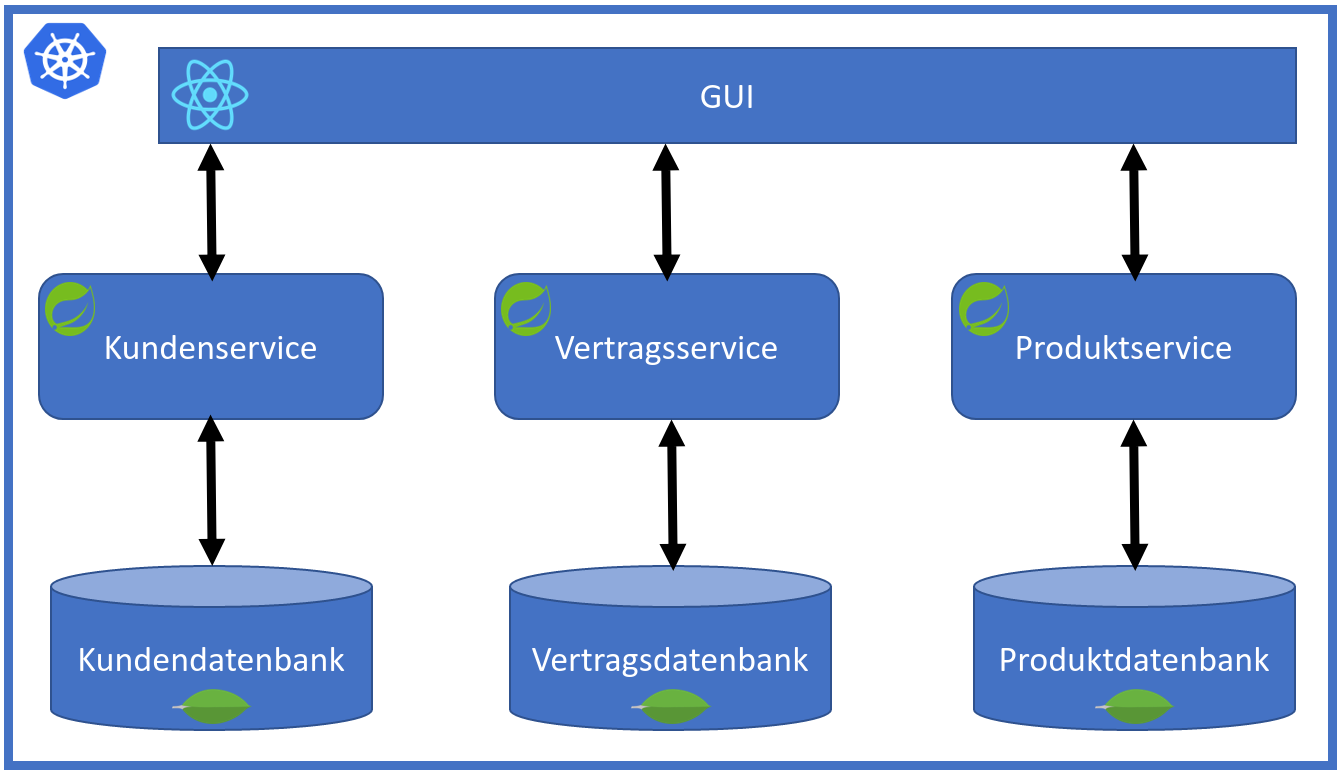
\includegraphics[width=0.95\textwidth]{figures/MicroCRM-Architecture.png}
    \caption{Grobkonzept CRM-System}
\end{figure}
Der letzte Abschnitt beinhaltet eine abschließende Betrachtung und Zusammenfassung der Arbeit.

\clearpage
\section{Vorläufige Gliederung}

\begin{outline}
	\item Einleitung
	\begin{outline}
		\item Motivation
		\item Zielsetzung
	\end{outline}
	\item Theoretischer Rahmen
	\begin{outline}
		\item DevOps
		\item Microservices
		\item Kubernetes
	\end{outline}
	\item Fallstudie
	\begin{outline}
		\item Problembeschreibung
		\item Entwurf
		\item Implementierung
		\item Bereitstellung
	\end{outline}
	\item Schlussbetrachtung
	\begin{outline}
		\item Fazit
		\item Ausblick
	\end{outline}
\end{outline}

\clearpage
\section{Zeitplan}

Im Folgenden wird ein grober Zeitplan angegeben. Die Bearbeitungszeit für die Bachelorarbeit beträgt drei Monate und somit ungefähr 13 Wochen.

\begin{figure}[H]
\centering
\begin{ganttchart}[
	vgrid,
	hgrid,
	x unit=0.8cm,
	bar/.append style={gray}
]{1}{13}
\gantttitle{Projektwochen}{13} \\
\gantttitlelist{1,...,13}{1} \\
\ganttmilestone{Anmeldung \enspace}{0} \ganttnewline 
\ganttbar{Einarbeitung}{1}{3} \ganttnewline 
\ganttmilestone{Endgültige Gliederung}{3} \ganttnewline
\ganttbar{Durchführung Fallstudie}{4}{9}  \ganttnewline 
\ganttmilestone{Fertige Fallstudie}{9} \ganttnewline
\ganttbar{Ausarbeitung Bachelorarbeit}{10}{13}  \ganttnewline
\ganttmilestone{Abgabe Bachelorarbeit}{13} \ganttnewline
\end{ganttchart}
\caption{Gantt-Diagramm}
\end{figure}

\clearpage
\begingroup
\setlength\bibitemsep{10pt}
\printbibheading
\printbibliography[type=book,title={Bücher},heading=subbibliography]
\printbibliography[type=inproceedings,title={Artikel},heading=subbibliography]
\endgroup

\end{document}